%--------------------------------------
% Create title frame
\titleframe

%--------------------------------------
% Table of contents
\begin{frame}{Overview}
  \setbeamertemplate{section in toc}[sections numbered]
  \tableofcontents[hideallsubsections]
\end{frame}

%--------------------------------------

\section{Introduction}

\begin{frame}{The current power system in ``developed'' countries}
    \begin{columns}
        \begin{column}{0.5\textwidth}
            \textbf{Pros :-)}
            \begin{itemize}
                \item Working seamlessly for decades
                \item Relatively affordable price
                \item High service level
            \end{itemize}
        \end{column}
        \begin{column}{0.5\textwidth}
            \textbf{Cons :-(}
            \begin{itemize}
              \item Relies heavily on hydrocarbons from extraction, that will inevitably vanish
              \item Difficulties to (re)develop Nuclear power
              \item Centralized, long distances, not always good for reliability and efficiency
              \item Public adoption issues for expansion
              \item hard to reproduce everywhere
              \item Difficulties to organize smarter distribution grids
            \end{itemize}
        \end{column}
    \end{columns}
\end{frame}

\begin{frame}
  \frametitle{}
  \centering \LARGE
  Can microgrids solve some of the cons while keeping the pros?

\end{frame}

\begin{frame}{A bit of history: Edison vs. Tesla}
  \begin{columns}
    \begin{column}{0.65\textwidth}      
      \begin{itemize}
        \item First grids followed Edison’s view, were DC and localized
        \item Tesla and co. imposed the bulk/centralized view in AC
        \begin{itemize}
          \item More adapted to motors
          \item Easier to raise/decrease voltage level, thus reduce losses
        \end{itemize}
        
        \item Now Edison view can be implemented because technically feasible:
        \begin{itemize}
          \item power electronics, energy storage, advanced load control, intelligent control, and communication
          \item (not necessarily through DC grids, although this could be an option).
        \end{itemize}
      \end{itemize}
    \end{column}
    \begin{column}{0.25\textwidth}
      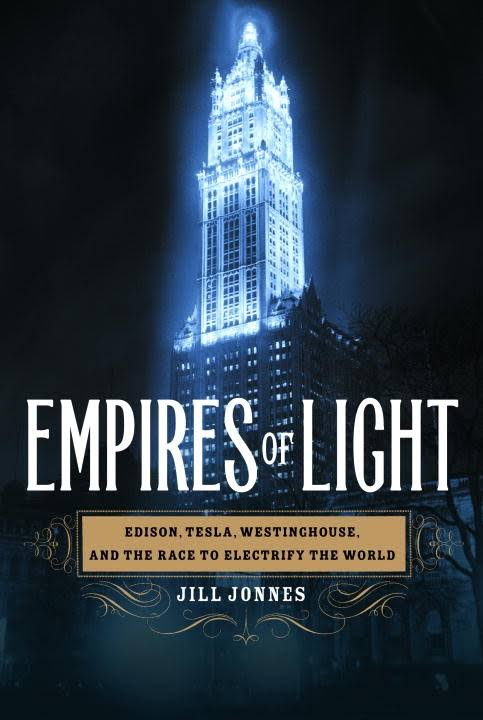
\includegraphics[width=\textwidth]{images/empires_of_light.jpg}
      \href{https://www.c-span.org/video/?178806-1/empires-light-edison-tesla-westinghouse}{Interview of the author}
    \end{column}
  \end{columns}
\end{frame}

\begin{frame}{First definition of a microgrid}
    A microgrid (MG) is a “complete” but small power system.

It is a network of consumer, generation and storage devices that can be optimized jointly to satisfy goals(*).

\begin{itemize}
  \item it can connect (be tied) to or disconnect (be islanded) from the main grid
\end{itemize}

It makes more sense when those devices are within clearly defined electrical boundaries.

It is on the “customer side”, although it can be operated by a third party.

*We will see later on what are the goals, or functions of a microgrid
\end{frame}

\begin{frame}{Components of a microgrid}
    \begin{columns}
        \begin{column}{0.6\textwidth}
            \begin{itemize}
                \item People
                \item Consumption devices
                \item Generation devices
                \item Storage devices
                \item Inverters
                \item A network
                \item Sensors and actuators
            \end{itemize}
        \end{column}
        \begin{column}{0.4\textwidth}
            %             \centering \textit{(Schematic Example)}
        \end{column}
    \end{columns}
\end{frame}

\begin{frame} {Schematic example}
  \centering
  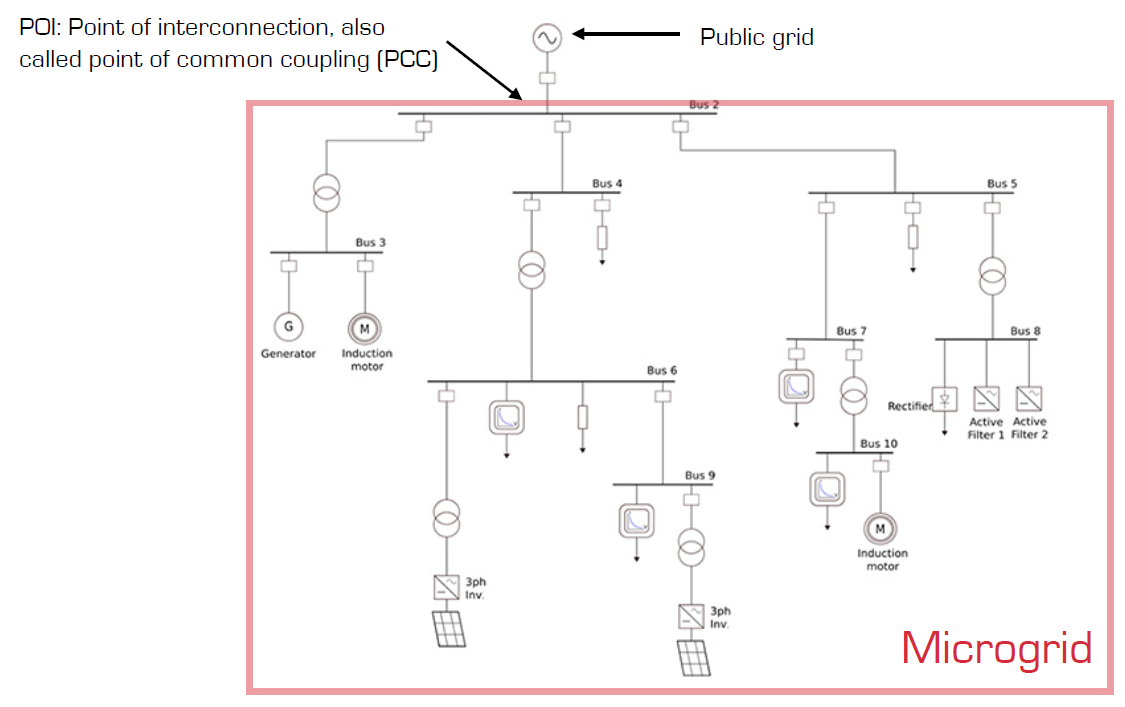
\includegraphics[width=0.7\textwidth]{images/microgrid_schematic_1.png} \\
  Source image taken from \href{https://www.typhoon-hil.com/}{Typhoon HIL webstite}
\end{frame}

\begin{frame}{``Copper plate'' assumption}
    In this course, unless stated otherwise, we (almost) neglect the network connecting the components of the microgrid.

This means mainly that we neglect losses, and other electrical phenomena that can be caused by the impedance of the cables connecting the devices.

Why?

\begin{itemize}
  \item Because network modeling is the topic of other courses (ELEC0447, ELEC0448).
  \item Because we will focus on other aspects not covered in these courses: MPPT, forecasting, operational planning, sizing.
\end{itemize}
\end{frame}

\begin{frame} {Schematically}
  \centering
  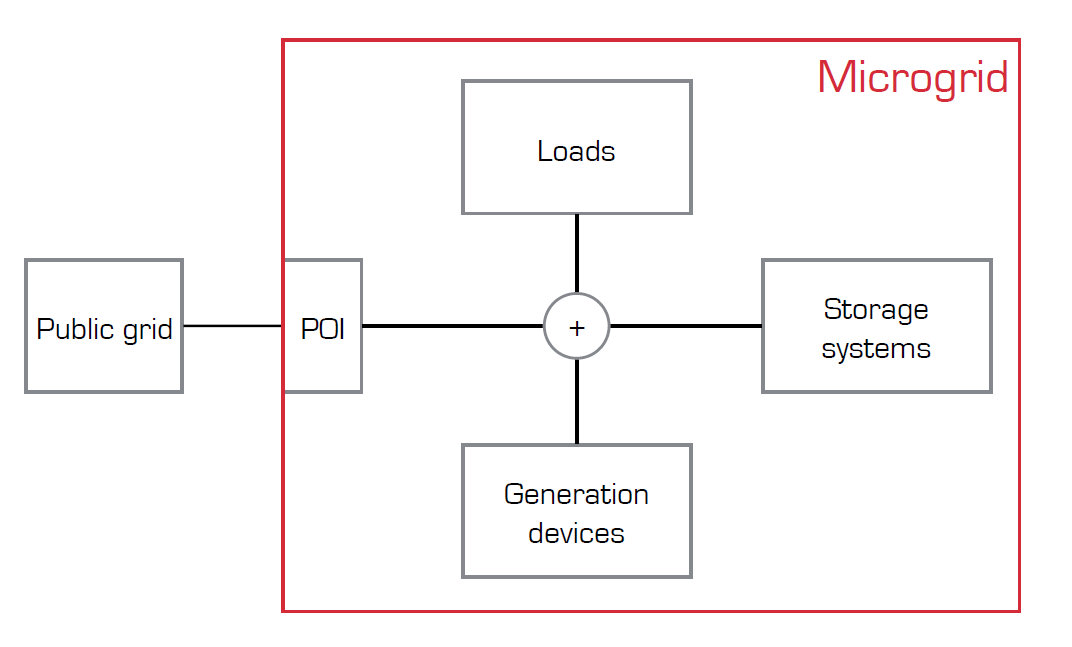
\includegraphics[width=0.8\textwidth]{images/microgrid_schematic_2.png}
\end{frame}

\begin{frame}{Main goals of a microgrid}

\begin{itemize}
  \item Satisfy the demand with maximum reliability and power quality
  \item Maximize the renewable energy harvested locally
  \item Minimise the total cost of electricity: local electricity may be cheaper than from the grid, at least periodically
  \item Help the public grid
  \item Local jobs, energy belongs to the people
  \item May increase security of supply, through (long-term) storage
\end{itemize}  
\end{frame}

\begin{frame}{Why building/studying microgrids?}

The
\begin{itemize}
  \item development of distributed generation,
  \item decreasing costs of storage means,
  \item evolution of communication and sensing technologies
\end{itemize}
open new options to the conventional distribution of electric energy and new possibilities for integrating distributed generation smoothly in constantly evolving energy and ancillary services markets (defined on the next slides).
\end{frame}

\begin{frame}[allowframebreaks]{Energy markets}
  \begin{columns}
    \begin{column}{0.45\textwidth}
      \begin{itemize}
        \item Energy markets organize the sales and purchases of the electricity commodity
        \item They are organized by time frame (futures, day-ahead, intra-day)
        \item By actively participating in the market, you can obtain the electricity at the price you are willing to pay or sell only if profitable.
      \end{itemize}    
    \end{column}    
    \begin{column}{0.53\textwidth}
        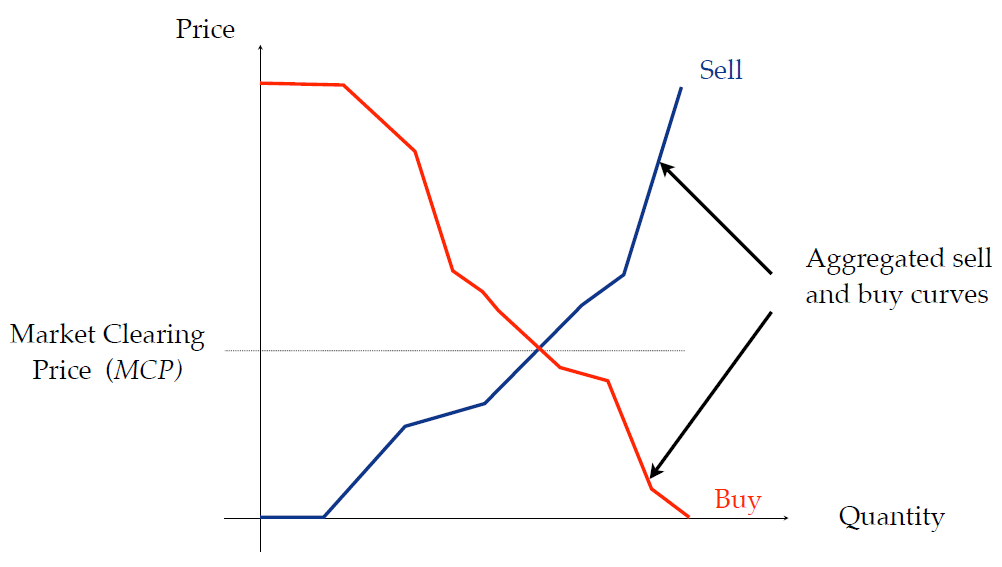
\includegraphics[width=\textwidth]{images/DAM.png}
    \end{column}

  \end{columns}
  
  \begin{itemize}
    \item Examples of market operators: Epex-Spot, NPS, ...
    \item Market operators, retailers and producers should not be confused with System operators (SOs):
    \begin{itemize}
      \item E.g. ELIA is the Belgian Transmission System Operator (TSO)
      \item E.g. Resa and ORES are Distribution System Operators (DSOs) in the Walloon region
    \end{itemize} 
    \item Microgrids are most of the time too small to access to the market. They’ll have to go through a “third party”, i.e. a retailer + balance responsible party (BRP)
  \end{itemize}
\end{frame}

\begin{frame}{Ancillary services markets}
Ancillary services are offered by entities that have the ability to modulate their generation or consumption, within prespecified boundaries and time frame, to help the system:
\begin{itemize}
  \item for balancing generation and demand
  \item for relieving congestions
  \item for voltage support
\end{itemize}
Ancillary services markets are organized by the TSO (e.g. ELIA in Belgium) for balancing services, and also by the DSO for local services (this is still a topic of active discussion)
\end{frame}


\begin{frame}{A (grid-tied) microgrid offers many value creation mechanisms}
\begin{center}
  
  \begin{tabularx}{\textwidth}{lXl}
    \toprule
    Function & Description & BSS\footnote{Battery Storage System.} \\
    \midrule
    Energy markets & Decide on the price your are willing to pay/sell & + \\
    Ancillary services & Sell services to the grid & ++ \\
    Peak reduction & Through local and community optimization & ++ \\
    UPS functionality & Operate in islanded mode & +++ \\
    Efficiency & Through optimized load and generation management & \\
    Community & Exchange energy locally at a preferred tariff & + \\
    \bottomrule
  \end{tabularx}
\end{center}

\end{frame}

\begin{frame}{Advantages for the public grid}
\begin{center}
  
  \begin{tabularx}{\textwidth}{Xl}
    \toprule
    Function & Description \\
    \midrule
    Peak reduction / flow management & Momentarily set constraints to the microgrid \\
    Voltage support & Reactive power flexibility of battery storage and PV \\
    Phase balancing & Using storage DC buffer \\
    Power factor correction & Flexibility of inverters \\
    Frequency support & Primary or secondary reserve \\
    \bottomrule
    \end{tabularx}
\end{center}

\end{frame}



\section{Special Cases}
\begin{frame}{Off-grid microgrids}
\begin{columns}
    \begin{column}{0.48\textwidth}
      Off-grid microgrids are a special case of microgrid.

      They have no connection to a public grid either because
      \begin{itemize}
        \item the public grid does not exist or cannot reach the location of the microgrid
        \item the public grid exists but is unreliable
      \end{itemize}    
    \end{column}    
    \begin{column}{0.5\textwidth}
        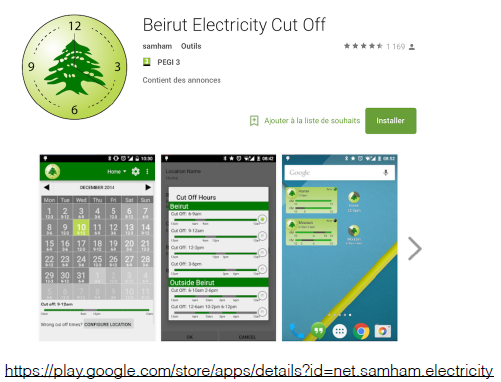
\includegraphics[width=\textwidth]{images/beirut.png}
    \end{column}

  \end{columns}
\end{frame}

\begin{frame}{Local Energy Communities}
\begin{columns}
    \begin{column}{0.55\textwidth}
      \begin{itemize}
        \item \alert{Single-user microgrid}: loads, generation, storage, a network, a connection to the grid (the definition of a micro-grid we have seen so far) Note: legal, e.g. your house with PV and storage.
        \item \alert{Community microgrid}: a group of single-user microgrids + a microgrid operator. Note: legal or not depending on the region you live in and the particular situation.
      \end{itemize}
    \end{column}    
    \begin{column}{0.4\textwidth}
        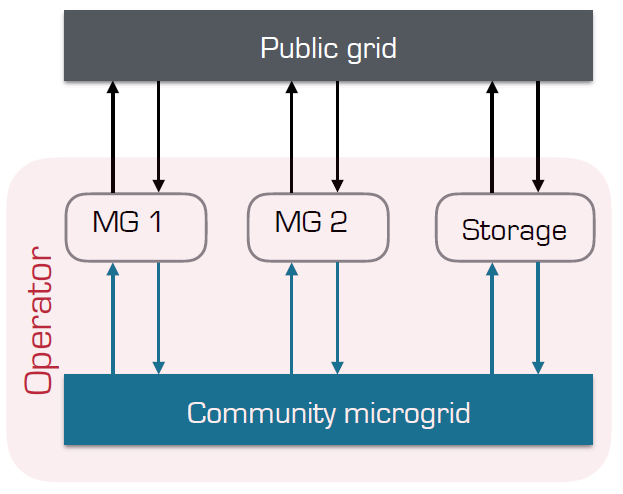
\includegraphics[width=\textwidth]{images/LEC.png}
    \end{column}
  \end{columns}
  Forming a local community allows reaching a critical size, but opens up other issues (regulatory, organizational, of fairness, etc.)  

\end{frame}

\begin{frame}{The MeryGrid project}
  
  \begin{center}
    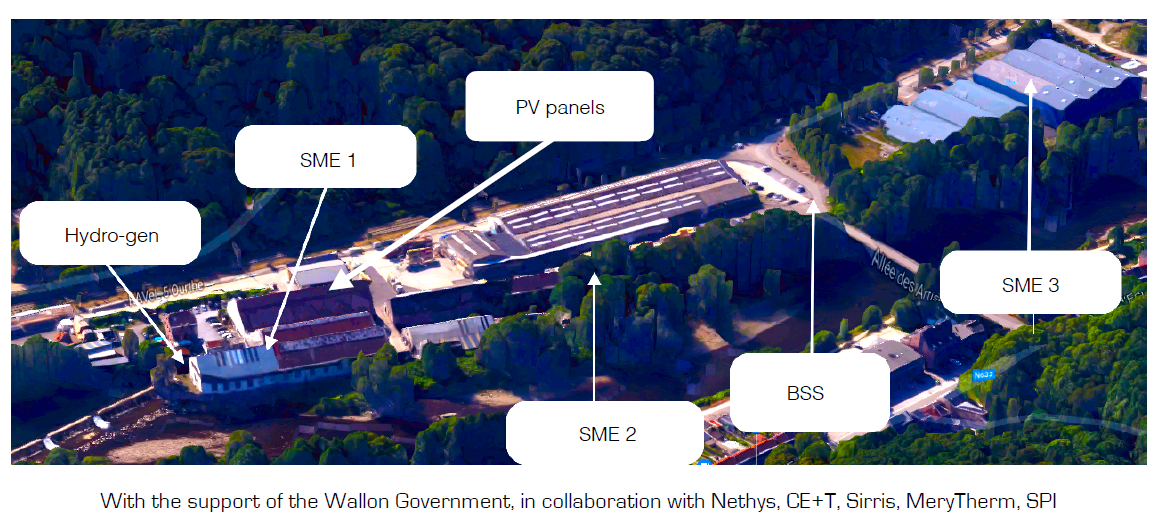
\includegraphics[width=0.7\textwidth]{images/merygrid.png}
  \end{center}
  
  \small \textit{Cornélusse, B., Ernst, D., Warichet, L., \& Legros, W. (2017). Efficient management of a connected microgrid in Belgium. In Proceedings of the 24th International Conference on Electricity Distribution, Glasgow, 12-15 June 2017. Available \href{https://orbi.uliege.be/handle/2268/211726}{here}.}
\end{frame}



\section{Microgrid Controllers}
\begin{frame}{Microgrid controllers}
  A microgrid controller is a software that is sensing the microgrid (currents, voltages, frequency, etc.) and taking control actions so as to operate safely, reliably and optimally the microgrid.

  In practice, a microgrid is run by multiple controllers, because there are several levels of control, which differ by their spatial and temporal scopes.

  Next to technological advances in production, consumption and storage, controllers are key elements for advanced microgrids.
\end{frame}

\begin{frame}{Control levels}
  
\begin{tabularx}{\textwidth}{llX} \toprule
Level & Function & Examples \\
\midrule
1 & Device level control & BSS control, reactive control, MPPT \\
2 & Local area control & Frequency regulation, fast load shedding \\
3 & Supervisory control & Forecasting, operational planning \\
4 & Public Grid interaction & Ancillary services, energy markets \\ \bottomrule
\end{tabularx}
  
\end{frame}

\begin{frame}[allowframebreaks]{Some functions of microgrid controllers}
Frequency control
\begin{itemize}
  \item balance generation and load => maintain frequency
  \item fast real-time, milli seconds
  \item Some predefined primary sources respond to frequency deviation (droop control)
\end{itemize}
Voltage control
\begin{itemize}
  \item Regulation of voltage a PCC within a respecified range (magnitude and phase)
  \item fast real-time, milli seconds
  \item Some predefined primary sources respond to voltage deviation (droop control)
\end{itemize}
Grid connected to islanded transition : intentional or unintentional
\begin{itemize}
  \item Islanded means MG keeps operating but is disconnected from main grid
  \item intentional means controller can prepare (e.g. start a genset, reduce current through PCC, etc.)
  \item unintentional means in reaction to a large disturbance, either internal or external to the MG
\end{itemize}
Islanded to grid-connected transition
\begin{itemize}
  \item MG resynchronizes and reconnects to the distribution system
\end{itemize}
Energy management: grid connected
\begin{itemize}
  \item Cf. all advantages offered by MG on previous slide
\end{itemize}
Energy management: islanded
\begin{itemize}
  \item “Economy mode” to power critical loads as long as possible
\end{itemize}
Microgrid protection
\begin{itemize}
  \item Configuration of protections of devices depending on operating conditions (e.g. islanded or not, a genes is up and running or not, etc.)
\end{itemize}
Microgrid black start
\begin{itemize}
  \item Restore islanded operation after complete shutdown
\end{itemize}
\end{frame}


\section{Organization}
\begin{frame}{Content of the course and evaluation}
\begin{itemize}
  \item Review microgrid components, technology and trends
  \item The main focus will be on design and optimal control of a microgrid
  \begin{itemize}
    \item Formulation of the associated control, optimization and machine learning problems
    \item With an introduction to the required mathematical background
    \item Detailed models of some components  
  \end{itemize}
  \item Evaluation:
  \item \begin{itemize}
    \item Maximum 5 mandatory assignments to practice all these concepts
    \item Small reports and oral presentations.
  \end{itemize}
\end{itemize}
\end{frame}

\begin{frame}{Important topics that are not covered in the course}
\begin{itemize}
  \item Detailed technical models and controllers of components (e.g. inverters):
  \begin{itemize}
    \item For energy storage, see CHIM0664-1 “Electrochemical energy conversion and storage” by Nathalie Job.
    \item For power electronics related topics, see ELEC0055-1 “Element of power Electronics”, by Fabrice Frebel
  \end{itemize}
  \item Organization of energy markets: ELEC0018-1 “Energy Markets” by Damien Ernst
  \item Protection devices and protection schemes
\end{itemize}
\end{frame}
